\subsection{YOLOv5}
\begin{frame}{}
    \LARGE Object Detection: \textbf{YOLOv5}
\end{frame}

\begin{frame}[allowframebreaks]{YOLOv5}
    \begin{figure}
        \centering
        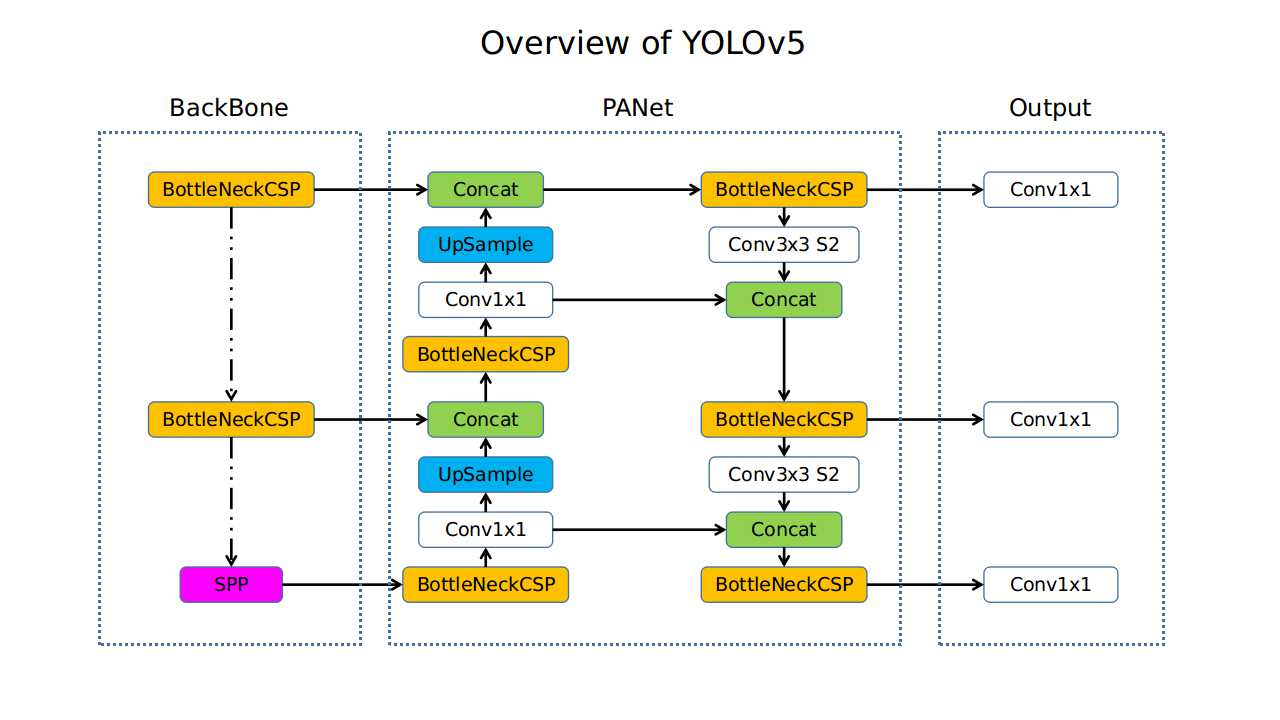
\includegraphics[width=1.0\textwidth,height=0.9\textheight,keepaspectratio]{images/object-detect/yolo-v5.png}
    \end{figure}
\framebreak
    \textbf{YOLOv5 (2020) Highlights:}
    \begin{itemize}
        \item Developed by Ultralytics with a PyTorch-based implementation.
        \item Offers multiple model sizes: nano (n), small (s), medium (m), large (l), extra-large (x).
        \item Introduces mosaic data augmentation for improved generalization.
        \item Achieves $\sim$49 mAP (COCO), $\sim$140 FPS (V100).
        \item Strengths: Easy to train, use, and deploy.
        \item Limitations: Still anchor-based; licensing under AGPL has faced scrutiny.
    \end{itemize}
\end{frame}